\documentclass[10pt,a4paper,twocolumn]{article}
\usepackage[T1]{fontenc}
\usepackage[utf8]{inputenc}
\usepackage{minted}
\usepackage{amsmath}
\usepackage{amsfonts}
\usepackage{amssymb}
\usepackage{fancyhdr}
\usepackage{graphicx, wrapfig, subcaption, setspace, booktabs}
\usepackage[font=small, labelfont=bf]{caption}
\usepackage[list=true]{subcaption}
\usepackage{url, lipsum}
\usepackage{hyperref}
\usepackage{listings}
\usepackage[dvipsnames]{xcolor}
\setlength\headheight{60pt}

\renewcommand{\figurename}{Figura}
\graphicspath{{figures/}}
\renewcommand{\headrulewidth}{2pt}
\definecolor{iselcolor}{rgb}{0.941,0.275 , 0.157} 
\definecolor{isel_beringela}{rgb}{0.37,0.08, 0.22} 
\renewcommand{\headrule}{\hbox to\headwidth{%
  \color{iselcolor}\leaders\hrule height \headrulewidth\hfill}}

\usepackage{lscape}

\renewcommand{\lstlistingname}{Algoritmo} % adjusts Listings caption and reference lst
\renewcommand{\lstlistlistingname}{Lista de Algoritmos}
\lstdefinelanguage{Kotlin}{
  comment=[l]{//},
  commentstyle={\color{gray}\ttfamily},
  emph={filter, first, firstOrNull, forEach, lazy, map, mapNotNull, println},
  emphstyle={\color{OrangeRed}},
  identifierstyle=\color{black},
  keywords={!in, !is, abstract, actual, annotation, as, as?, break, by, catch, class, companion, const, constructor, continue, crossinline, data, delegate, do, dynamic, else, enum, expect, external, false, field, file, final, finally, for, fun, get, if, import, in, infix, init, inline, inner, interface, internal, is, lateinit, noinline, null, object, open, operator, out, override, package, param, private, property, protected, public, receiveris, reified, return, return@, sealed, set, setparam, super, suspend, tailrec, this, throw, true, try, typealias, typeof, val, var, vararg, when, where, while},
  keywordstyle={\color{NavyBlue}\bfseries},
  morecomment=[s]{/*}{*/},
  morestring=[b]",
  morestring=[s]{"""*}{*"""},
  ndkeywords={@Deprecated, @JvmField, @JvmName, @JvmOverloads, @JvmStatic, @JvmSynthetic, Array, Byte, Double, Float, Int, Integer, Iterable, Long, Runnable, Short, String, Any, Unit, Nothing},
  ndkeywordstyle={\color{BurntOrange}\bfseries},
  sensitive=true,
  stringstyle={\color{ForestGreen}\ttfamily},
}

\begin{document}
\pagestyle{fancy}
\fancyhead{} % clear all header fields
\fancyhead[LO]{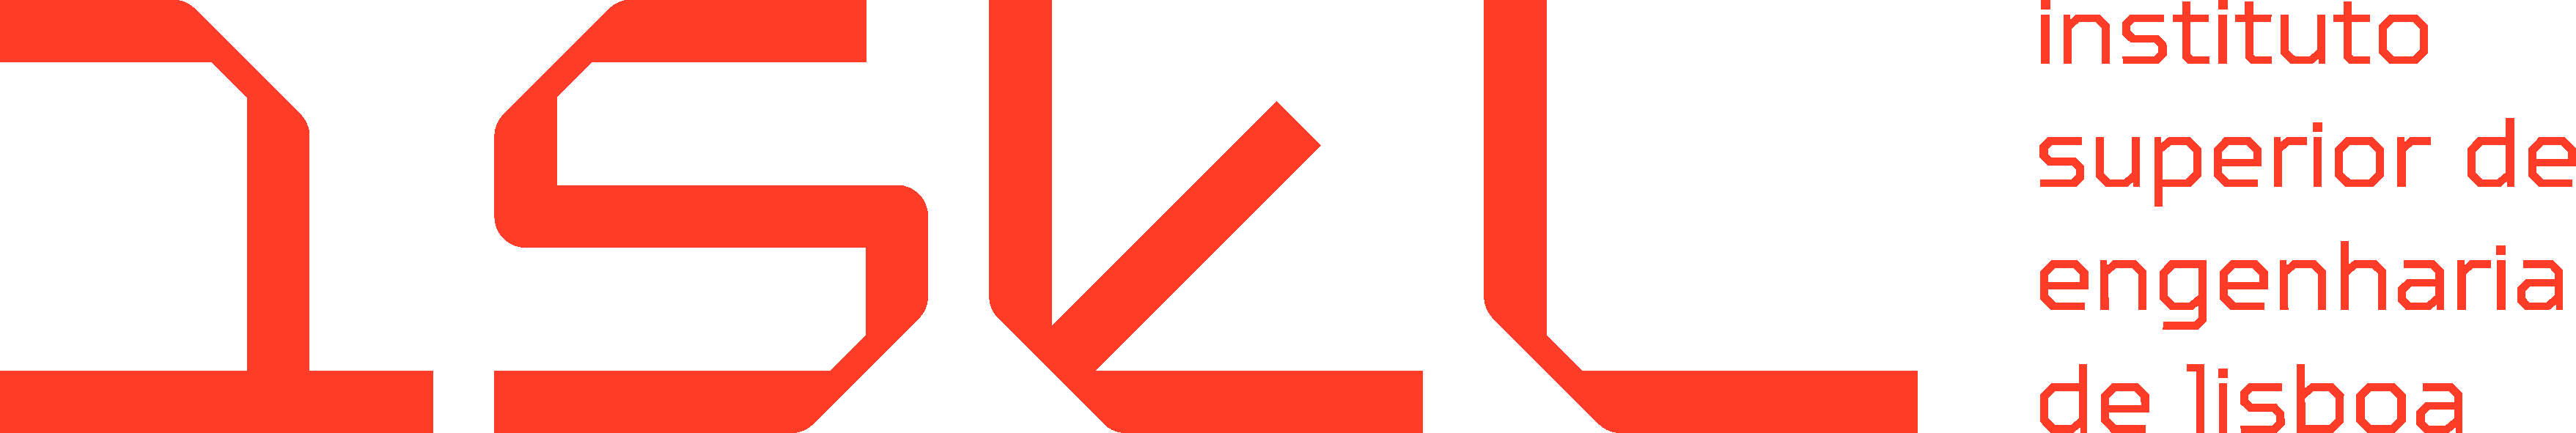
\includegraphics[width=4cm]{01_ISEL-Logotipo-RGB_Horizontal-Compacto-900.png}}
\fancyhead[RO]{
\textbf{Keyboard Reader} (\textit{Ticket Machine}) \\ 
\footnotesize
Laboratório de Informática e Computadores 2025 / 2026 verão \\
Autores: Hugo Gomes / José Gaspar / Rafael Hipólito}
\fancyfoot{} % clear all footer fields
\fancyfoot[RO]{\thepage}


O módulo \textit{Keyboard Reader }é constituído por três blocos principais, de acordo com o diagrama representado 
na Figura \ref{fig:keyboardReader}:

\textit{i}) o descodificador de teclado (\textit{Key Decode});

\textit{ii}) o bloco de armazenamento (designado por \textit{Ring Buffer});

\textit{iii}) o bloco de entrega ao consumidor (designado por \textit{Key Transmitter}).

Neste caso o módulo \textit{Control}, implementado em software, é a entidade consumidora.

\begin{figure}[!h]
\begin{center}
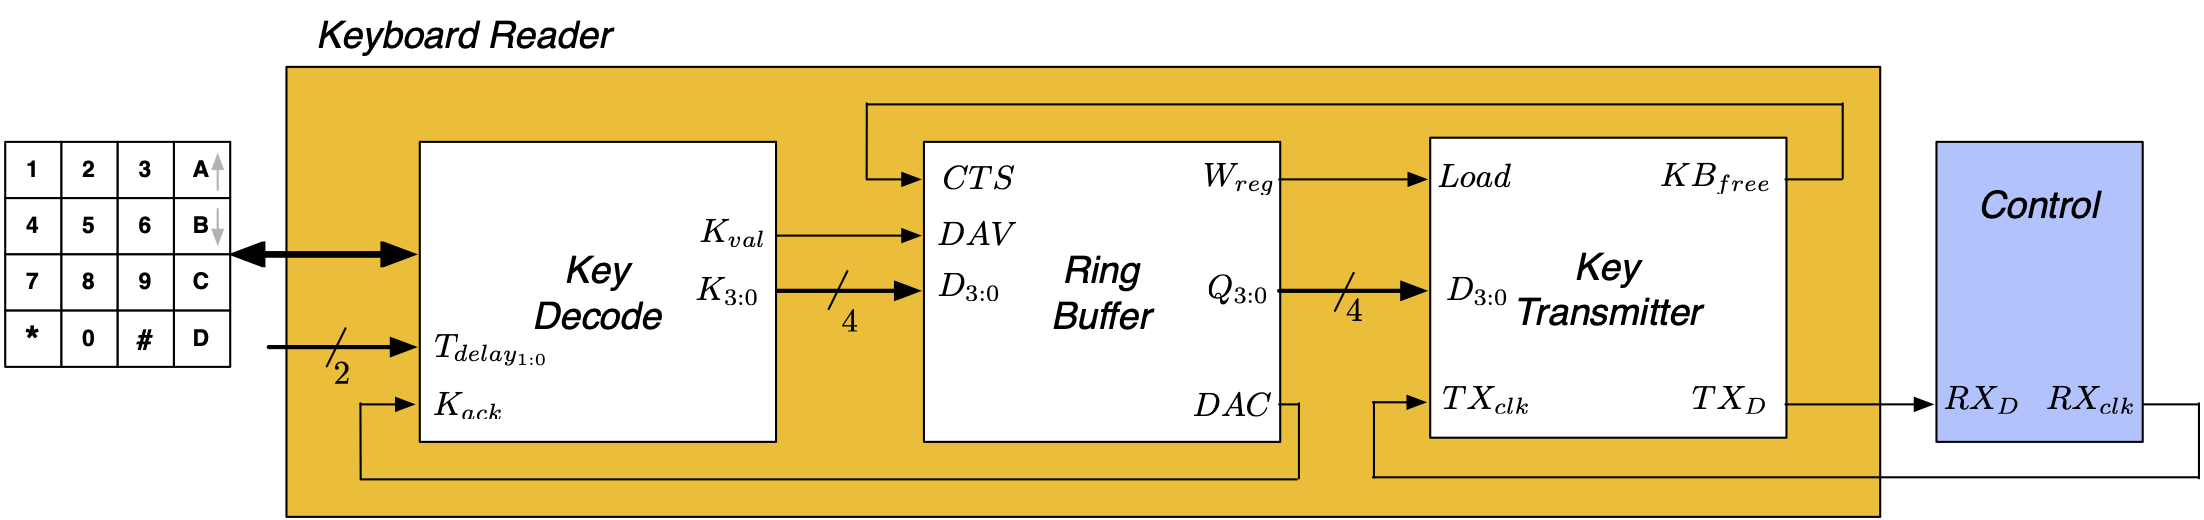
\includegraphics[width=0.48\textwidth]{keyboardReader_diagram.png} 
\caption{Diagrama de blocos do módulo \textit{Keyboard Reader}}
\label{fig:keyboardReader}
\end{center}
\end{figure} 

\section{Key Decode}

\noindent \par O bloco \textit{Key Decode} implementa um descodificador de um teclado matricial 4x4 em hardware, sendo
constituído por três sub-blocos, conforme o diagrama de blocos representado na Figura~\ref{fig:keyDecode_diagram}:

\textit{i}) uma ligação ao teclado matricial 4x4, da placa de expansão fornecida;

\textit{ii}) o bloco \textit{Key Scan}, responsável pelo varrimento do teclado;

\textit{iii}) o bloco \textit{Key Control}, que realiza o controlo do varrimento e o controlo de fluxo

O controlo de fluxo de saída do bloco \textit{Key Decode} (para o módulo \textit{Key Buffer}), define que
o sinal $K_{val}$ é ativado quando é detetada a pressão de uma tecla, sendo também disponibilizado o 
código dessa tecla no \textit{bus} $K_{3:0}$. Por ordem, do \textit{bit} mais significativo para o menos, o código da tecla premida
corresponde à coluna, seguida da linha, cada informação com 2 \textit{bits}.
Apenas é iniciado um novo ciclo de varrimento ao teclado quando o sinal $K_{ack}$ for ativado. 
O diagrama temporal do controlo de fluxo está representado na Figura~\ref{fig:keyDecode_protocol}.

\begin{figure}[!h]
\centering
\begin{subfigure}{0.5\textwidth}
	\centering
	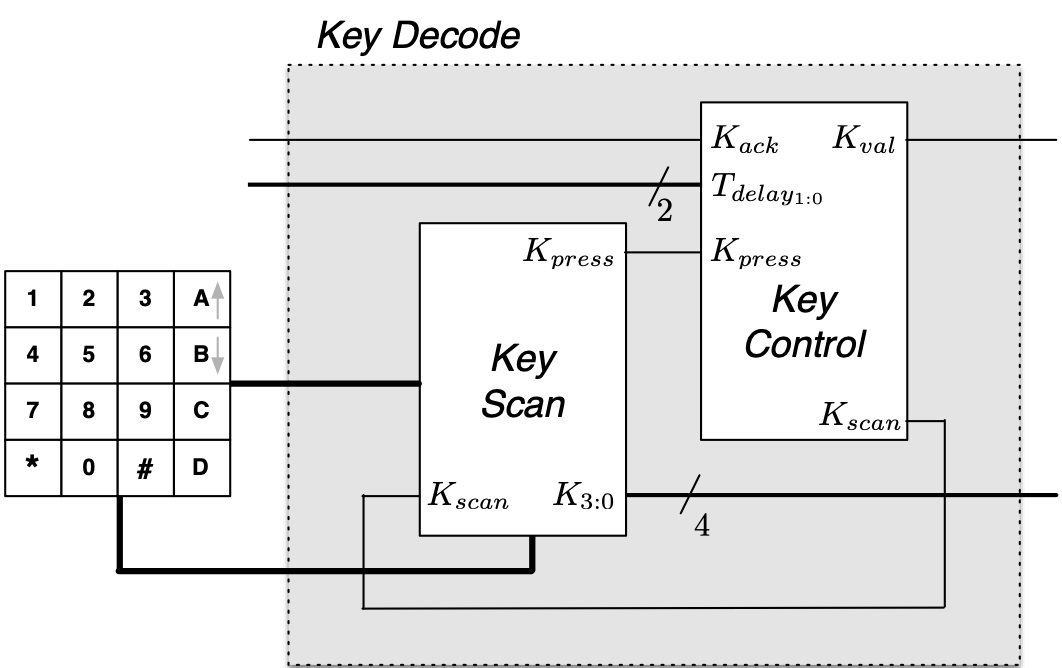
\includegraphics[width=0.70\textwidth]{keyDecode_architecture.png} 
    \caption{Diagrama de blocos}
    \label{fig:keyDecode_diagram}
\end{subfigure}
\begin{subfigure}{0.5\textwidth}
	\centering
	\includegraphics[width=0.50\textwidth]{keydecode_protocol.png} 
    \caption{Diagrama temporal}
    \label{fig:keyDecode_protocol}
\end{subfigure}
\caption{Bloco \textit{Key Decode}}
\label{fig:keyDecode}
\end{figure}

\subsection{Key Scan}

\noindent \par O bloco \textit{Key Scan} foi implementado de acordo com o diagrama de blocos representado na Figura~\ref{fig:keyScan}.

O diagrama do bloco KeyScan da Figura \ref{fig:keyScan} corresponde à 3ª versão da possível implementação, de três 
disponibilizadas pelos docentes.

Foi escolhida esta opção com a utilização de um \textit{priority encoder} (\textit{PENC}) pois este permite uma leitura mais rápida e
eficiente do teclado.

Este componente permite a ativação imediata do sinal $K_{press}$ assim que é detetada uma tecla 
pressionada, reduzindo a latência de resposta do sistema. Adicionalmente, assegura a priorização de linhas de maior ordem 
(inferiores) quando múltiplas teclas são pressionadas na mesma coluna, garantindo um comportamento determinístico.

\begin{figure}[H]
\begin{center}
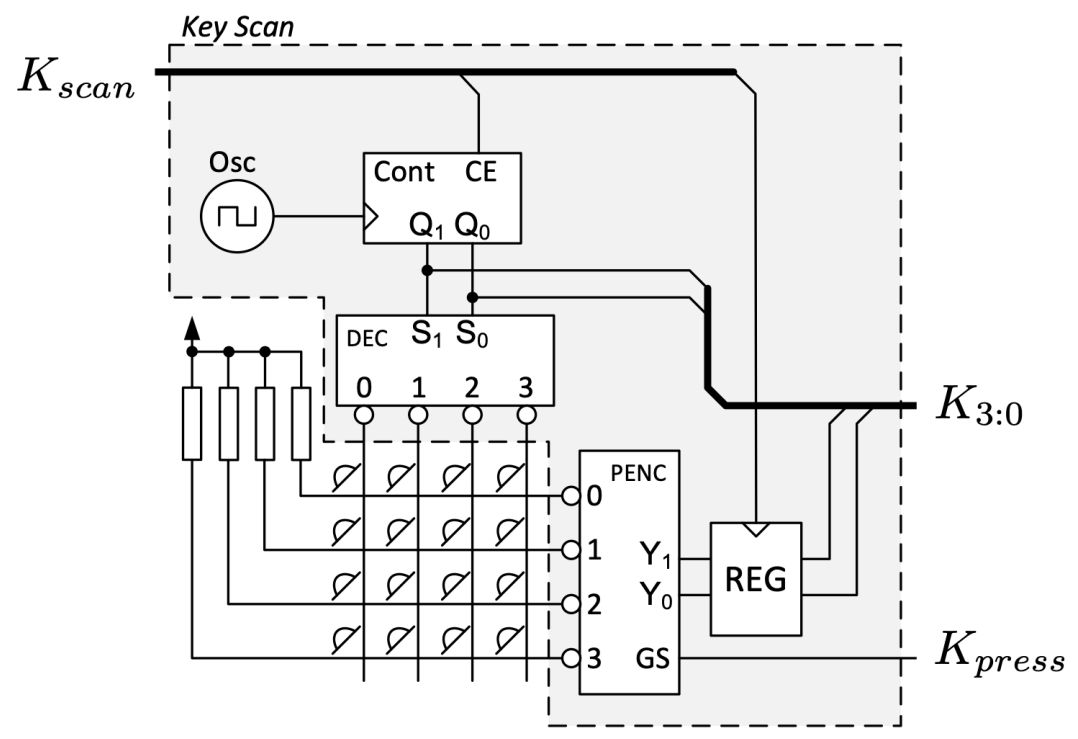
\includegraphics[width=0.30\textwidth]{keyScan_diagrama_blocos.jpg} 
\caption{Diagrama de blocos do módulo \textit{Key Scan}}
\label{fig:keyScan}
\end{center}
\end{figure} 

\subsection{Key Control}

\noindent \par O bloco \textit{Key Control} foi implementado pela máquina de estados representada em \textit{ASM-chart}
na Figura~\ref{fig:keyControl_ASM}.

A nossa solução de implementação da máquina de estados, correspondente ao bloco \textit{Key Control}, consiste na criação de 3 estados:

\begin{itemize}
  \item \textit{Scanning}: Ativa a saída $K_{scan}$, que indica que o varrimento do teclado está a ser feito, aguardando por 
  uma tecla ser premida. Após uma tecla ser premida ($K_{press}$ assume o valor lógico 1, correspondente a \textit{True}), a máquina avança para o estado seguinte.
  \item \textit{Sending}: Este estado envia a indicação de tecla premida, através de $K_{val}$. Quando a tecla premida é 
  consumida pelo \textit{Ring Buffer}, este envia um sinal com essa indicação, $K_{ack}$, que faz o controlador mudar de estado.
  \item \textit{Acknowledged}: Após a tecla ser consumida pelo \textit{Ring Buffer}, este estado aguarda, independentemente de 
  outra tecla ser premida, a transição descendente de $K_{ack}$ que, caso outra tecla seja premida ($K_{press}$ com valor 
  lógico '1'), envia a máquina para o estado \textit{Sending}. Caso não seja premida outra tecla, com a transição descendente de 
  $K_{ack}$, a máquina volta para o estado inicial \textit{Scanning}, aguardando que outra tecla seja premida.
\end{itemize}

Esta implementação, em particular após o último estado, foi feita tendo em conta, numa fase futura, a adição de \textit{Tdelay}, que premite o pressionamento de outra tecla após a primeira ter sido registada.

A descrição hardware do bloco \textit{Key Decode} em\textit{ VHDL} encontra-se no Anexo~\ref{vhdl:KeyDecode}.

\begin{figure}[H]
\begin{center}
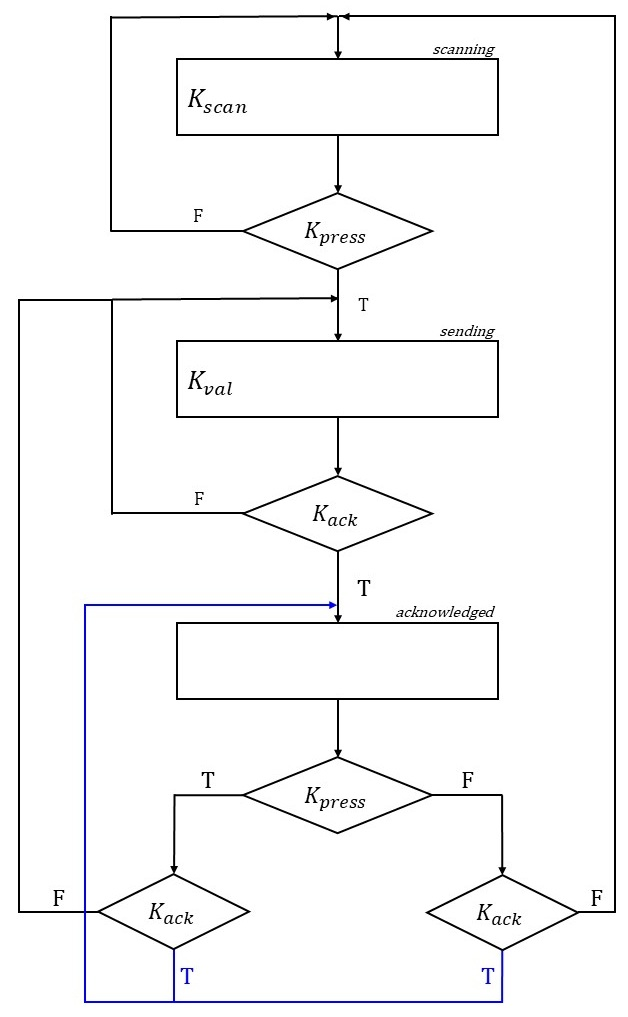
\includegraphics[width=0.40\textwidth]{keyControl_ASM.jpg} 
\caption{Máquina de estados do \textit{Key Control}}
\label{fig:keyControl_ASM}
\end{center}
\end{figure} 


\section{Conclusões}

\noindent \par Este componente, \textit{Keyboard Reader}, é responsável pela leitura do teclado, na parte de \textit{hardware},
através de um contador para varrer cada coluna e de um \textit{Priority Encoder} para varrer cada linha.

Quando uma tecla é premida, o varrimento de linhas e colunas é parado e estas são registadas, em $K_{3:0}$.
Existe também uma variável, $K_{val}$, que indica que existe um valor a ser registado. Estes valores são, 
atualmente, enviados para o \textit{USBPort}, que o transmite do \textit{hardware} para o \textit{software}.

No \textit{software}, através do objeto \textit{KBD}, é lida a posição, linha e coluna, passada pelo
\textit{hardware} e, através de uma matriz definida no objeto, é devolvida a informação, pela função
\textit{getKey()}, da tecla que foi premida.

\onecolumn
\newpage
\section*{Referências}
\addcontentsline{toc}{section}{\protect\numberline{}Referências}
\begin{thebibliography}{9}
\bibitem{Slides das aulas}
Laboratório de Informática e Computadores - Slides de apoio às aulas, 2025/2026.

\bibitem{Enunciado}
Laboratório de Informática e Computadores - Enunciado do Projeto "Ticket Machine", 2025/2026.

\bibitem{guiaQuartus}
Pedro Miguens Matutino, Sérgio André \emph{Guia de Instalação do Quartus Prime Lite Edition 20.1.1.720}, 2022, ISEL.
\end{thebibliography}

\clearpage
\appendix
\section{VHDL}

\subsection{Keyboard Reader}
\label{sec:KbdReader_VHDL}
\begin{minipage}[H]{\linewidth}
\footnotesize
\inputminted{vhdl}{vhdl/keyboardReader.vhd}
\label{vhdl:KbdReader}
\end{minipage}

\subsection{Keyboard Reader testbench}
\label{sec:KbdReader_tb_VHDL}
\begin{minipage}{\linewidth}
\footnotesize
\inputminted{vhdl}{vhdl/keyboardReader_tb.vhd}
\label{vhdl:KbdReader_tb}
\end{minipage}

\subsection{Key Decode}
\label{sec:KeyDecode_VHDL}
\begin{minipage}{\linewidth}
\footnotesize
\inputminted{vhdl}{vhdl/KeyDecode.vhd}
\label{vhdl:KeyDecode}
\end{minipage}

\subsection{Key Decode testbench}
\label{sec:KeyDecode_tb_VHDL}
\begin{minipage}{\linewidth}
\footnotesize
\inputminted{vhdl}{vhdl/KeyDecode_tb.vhd}
\label{vhdl:KeyDecode_tb}
\end{minipage}

\subsection{Key Scan}
\label{sec:KeyScan_VHDL}
\begin{minipage}{\linewidth}
\footnotesize
\inputminted{vhdl}{vhdl/KeyScan.vhd}
\label{vhdl:KeyScan}
\end{minipage}

\subsection{Key Scan testbench}
\label{sec:KeyScan_tb_VHDL}
\begin{minipage}{\linewidth}
\footnotesize
\inputminted{vhdl}{vhdl/KeyScan_tb.vhd}
\label{vhdl:KeyScan_tb}
\end{minipage}

\subsection{Counter}
\label{sec:Counter_VHDL}
\begin{minipage}{\linewidth}
\footnotesize
\inputminted{vhdl}{vhdl/Counter.vhd}
\label{vhdl:Counter}
\end{minipage}

\subsection{Counter testbench}
\label{sec:Counter_tb_VHDL}
\begin{minipage}{\linewidth}
\footnotesize
\inputminted{vhdl}{vhdl/Counter_tb.vhd}
\label{vhdl:Counter_tb}
\end{minipage}

\subsection{Adder}
\label{sec:Adder_VHDL}
\begin{minipage}{\linewidth}
  \footnotesize
  \inputminted{vhdl}{vhdl/Adder.vhd}
  \label{vhdl:Adder}
\end{minipage}

\subsection{FA}
\label{sec:FA_VHDL}
\begin{minipage}{\linewidth}
\footnotesize
\inputminted{vhdl}{vhdl/FA.vhd}
\label{vhdl:FA}
\end{minipage}

\subsection{HA}
\label{sec:HA_VHDL}
\begin{minipage}{\linewidth}
\footnotesize
\inputminted{vhdl}{vhdl/HA.vhd}
\label{vhdl:HA}
\end{minipage}

\subsection{RG2}
\label{sec:RG2_VHDL}
\begin{minipage}{\linewidth}
  \footnotesize
  \inputminted{vhdl}{vhdl/RG2.vhd}
  \label{vhdl:RG2}
\end{minipage}

\subsection{Decoder}
\label{sec:Decoder_VHDL}
\begin{minipage}{\linewidth}
\footnotesize
\inputminted{vhdl}{vhdl/Decoder.vhd}
\label{vhdl:Decoder}
\end{minipage}

\subsection{Decoder testbench}
\label{sec:Decoder_tb_VHDL}
\begin{minipage}{\linewidth}
\footnotesize
\inputminted{vhdl}{vhdl/Decoder_tb.vhd}
\label{vhdl:Decoder_tb}
\end{minipage}

\subsection{DeMUX}
\label{sec:DeMUX_VHDL}
\begin{minipage}{\linewidth}
\footnotesize
\inputminted{vhdl}{vhdl/DeMUX.vhd}
\label{vhdl:DeMUX}
\end{minipage}

\subsection{PEnc 4:2}
\label{sec:PEnc42_VHDL}
\begin{minipage}{\linewidth}
\footnotesize
\inputminted{vhdl}{vhdl/Decoder.vhd}
\label{vhdl:PEnc42}
\end{minipage}

\subsection{PEnc}
\label{sec:PEnc_VHDL}
\begin{minipage}{\linewidth}
\footnotesize
\inputminted{vhdl}{vhdl/PEnc.vhd}
\label{vhdl:PEnc}
\end{minipage}

\subsection{Key Control}
\label{sec:KeyControl_VHDL}
\begin{minipage}{\linewidth}
\footnotesize
\inputminted{vhdl}{vhdl/KeyControl.vhd}
\label{vhdl:KeyControl}
\end{minipage}

\subsection{Key Control testbench}
\label{sec:KeyControl_tb_VHDL}
\begin{minipage}{\linewidth}
\footnotesize
\inputminted{vhdl}{vhdl/KeyControl_tb.vhd}
\label{vhdl:KeyControl_tb}
\end{minipage}

\subsection{FFD}
\label{sec:FFD_VHDL}
\begin{minipage}{\linewidth}
\footnotesize
\inputminted{vhdl}{vhdl/FFD.vhd}
\label{vhdl:FFD}
\end{minipage}

\clearpage
\section{\textit{Kotlin}}
\subsection{HAL}
\lstinputlisting[language=Kotlin, basicstyle=\scriptsize, caption={HAL - Hardware Abstract Layer}, label={lst:HAL}]{kotlin/HAL.kt}


\subsection{KBD}
\lstinputlisting[language=Kotlin, basicstyle=\scriptsize, caption={KBD}, label={lst:KBD}]{kotlin/KBD.kt}


\end{document}